% !Mode:: "TeX:UTF-8"

\chapter{绪论}
\label{sec:intro}
\section{研究背景及意义}
% \textcolor{red}{正文大概12/65页,最后需要调整一遍格式}

% \textcolor{red}{问题用红色标出,重复用蓝色标出}

% \textcolor{red}{简要说明此项研究工作的目的意义、范围、相关领域的国内外研究现状及前人研究情况和成果(或属知识空白)、理论分析及依据、研究设想、研究方法等,一般不超过全文篇幅的15%。}

% 图的大小一般为宽6.67×高5.00cm。特殊情况下,也可宽9.00×高6.75cm,或宽13.5×高9.00cm。总之,一篇论文中,同类图片的大小应该一致,编排美观、整齐。

% 四号14pt 小四12pt 五号10.5pt

% 图中的标目是说明坐标轴物理意义的项目,它是由物理量的符号或名称和相应的单位组成。物理量的符号由斜体字母标注,单位的符号使用正体字母标注,量与单位间用斜线隔开。例如:ρ/kg•m-3 ,/MPa,E/GPa  等等。(目前存在一些问题)
% (4)图中用字为五号(10.5pt),如排列过密,用五号字有困难时,可小于五号字,但不得小于七号字。


% 一律使用三线表,与文字齐宽,线粗1磅。

% 据此 进行 以及
% NOTE: 问题用红色标出
在现代电子战信息获取和处理技术中,雷达信号识别分类是一个十分重要的方面。它主要指的是利用雷达、声波探测等各种主动、被动传感器获取信号,基于此感知识别周围环境信息并检测识别出感兴趣的目标。

天波超视距雷达(简称天波雷达, OTHR)利用电磁波在电离层间的反射传输高频能量,具有反隐身、抗干扰等优点,其预警能力远远超出常规体制雷达,从而受到越来越多国家的关注。
但是由于天波量测与目标状态所在坐标系的不统一以及无法实时获得准确的坐标配准系数,导致天波雷达的目标定位精度较差。
通过地海杂波识别技术获得地理轮廓与实际地理位置进行匹配,可辨识坐标配准系数,进而提高目标定位精度。

雷达辐射源识别的主要目的是详细地了解信号环境中所有雷达信号的特征参数,从中进一步判断这些雷达的用途、平台类别,进而判断其武器系统及威胁等级,为战略情报分析提供信息\ucite{matuszewski2008specific}。
通过雷达辐射源个体识别,可以对战场环境中敌我双方雷达辐射源的分布情况实施侦察,以提供更加全面精确的电磁斗争态势,
从而进行有效的战场指挥与决策。
然而由于辐射源的特征未知、信号波形日趋复杂、战时电磁环境恶劣等原因,辐射源的精确识别面临越来越严峻的挑战。

本文基于上述两个雷达信号分类识别问题,对实际数据进行分析,利用深度学习方法,对天波雷达地海杂波识别以及辐射源识别进行研究分析,对雷达信号的分类研究具有一定的工程意义。

\section{研究现状}
\subsection{天波雷达地海杂波识别研究现状}
天波雷达利用电磁波在电离层与地面或者海面之间的反射作用传输高频能量,其作用距离不受地球曲率的限制,可实现对隐身战斗机、洲际导弹、巡航导弹和大中型舰船等高价值目标的远程预警,受到世界各国的高度关注。
天波雷达的主要工作原理如图\ref{fig:othr_how}所示,其工作频率为6-28MHz,通过电离层反射作用来检测和定位1000~公里到3000~公里范围内(地平线以下)的飞机、地面或者海洋目标,因此在持续监测中起着重要作用\ucite{headrick1974over, fabrizio2013high}。
然而,电磁信号通过电离层的传播会产生坐标系转换问题。目标处于大地坐标系(即经度和纬度),而天波雷达接收的量测信号定义在雷达坐标系下(即斜距和方位角)\ucite{krolik1997maximum},这给雷达的目标跟踪与定位提出了新的处理步骤:坐标配准。
坐标配准是将天波雷达目标从雷达坐标系转换到地理坐标系的过程。天波雷达的坐标配准在很大程度上影响着雷达跟踪精度,尤其是对电离层参数无法精确、实时获得的较远的区域。
如果在雷达坐标系进行目标跟踪,整个坐标配准的过程可以分为两个子过程:
(1)为每个量测或目标状态估计选择正确的电离层传播模式;
(2)将量测或目标的状态估计从雷达坐标系转换为大地坐标系。
\begin{figure}[hbt]
	\centering
	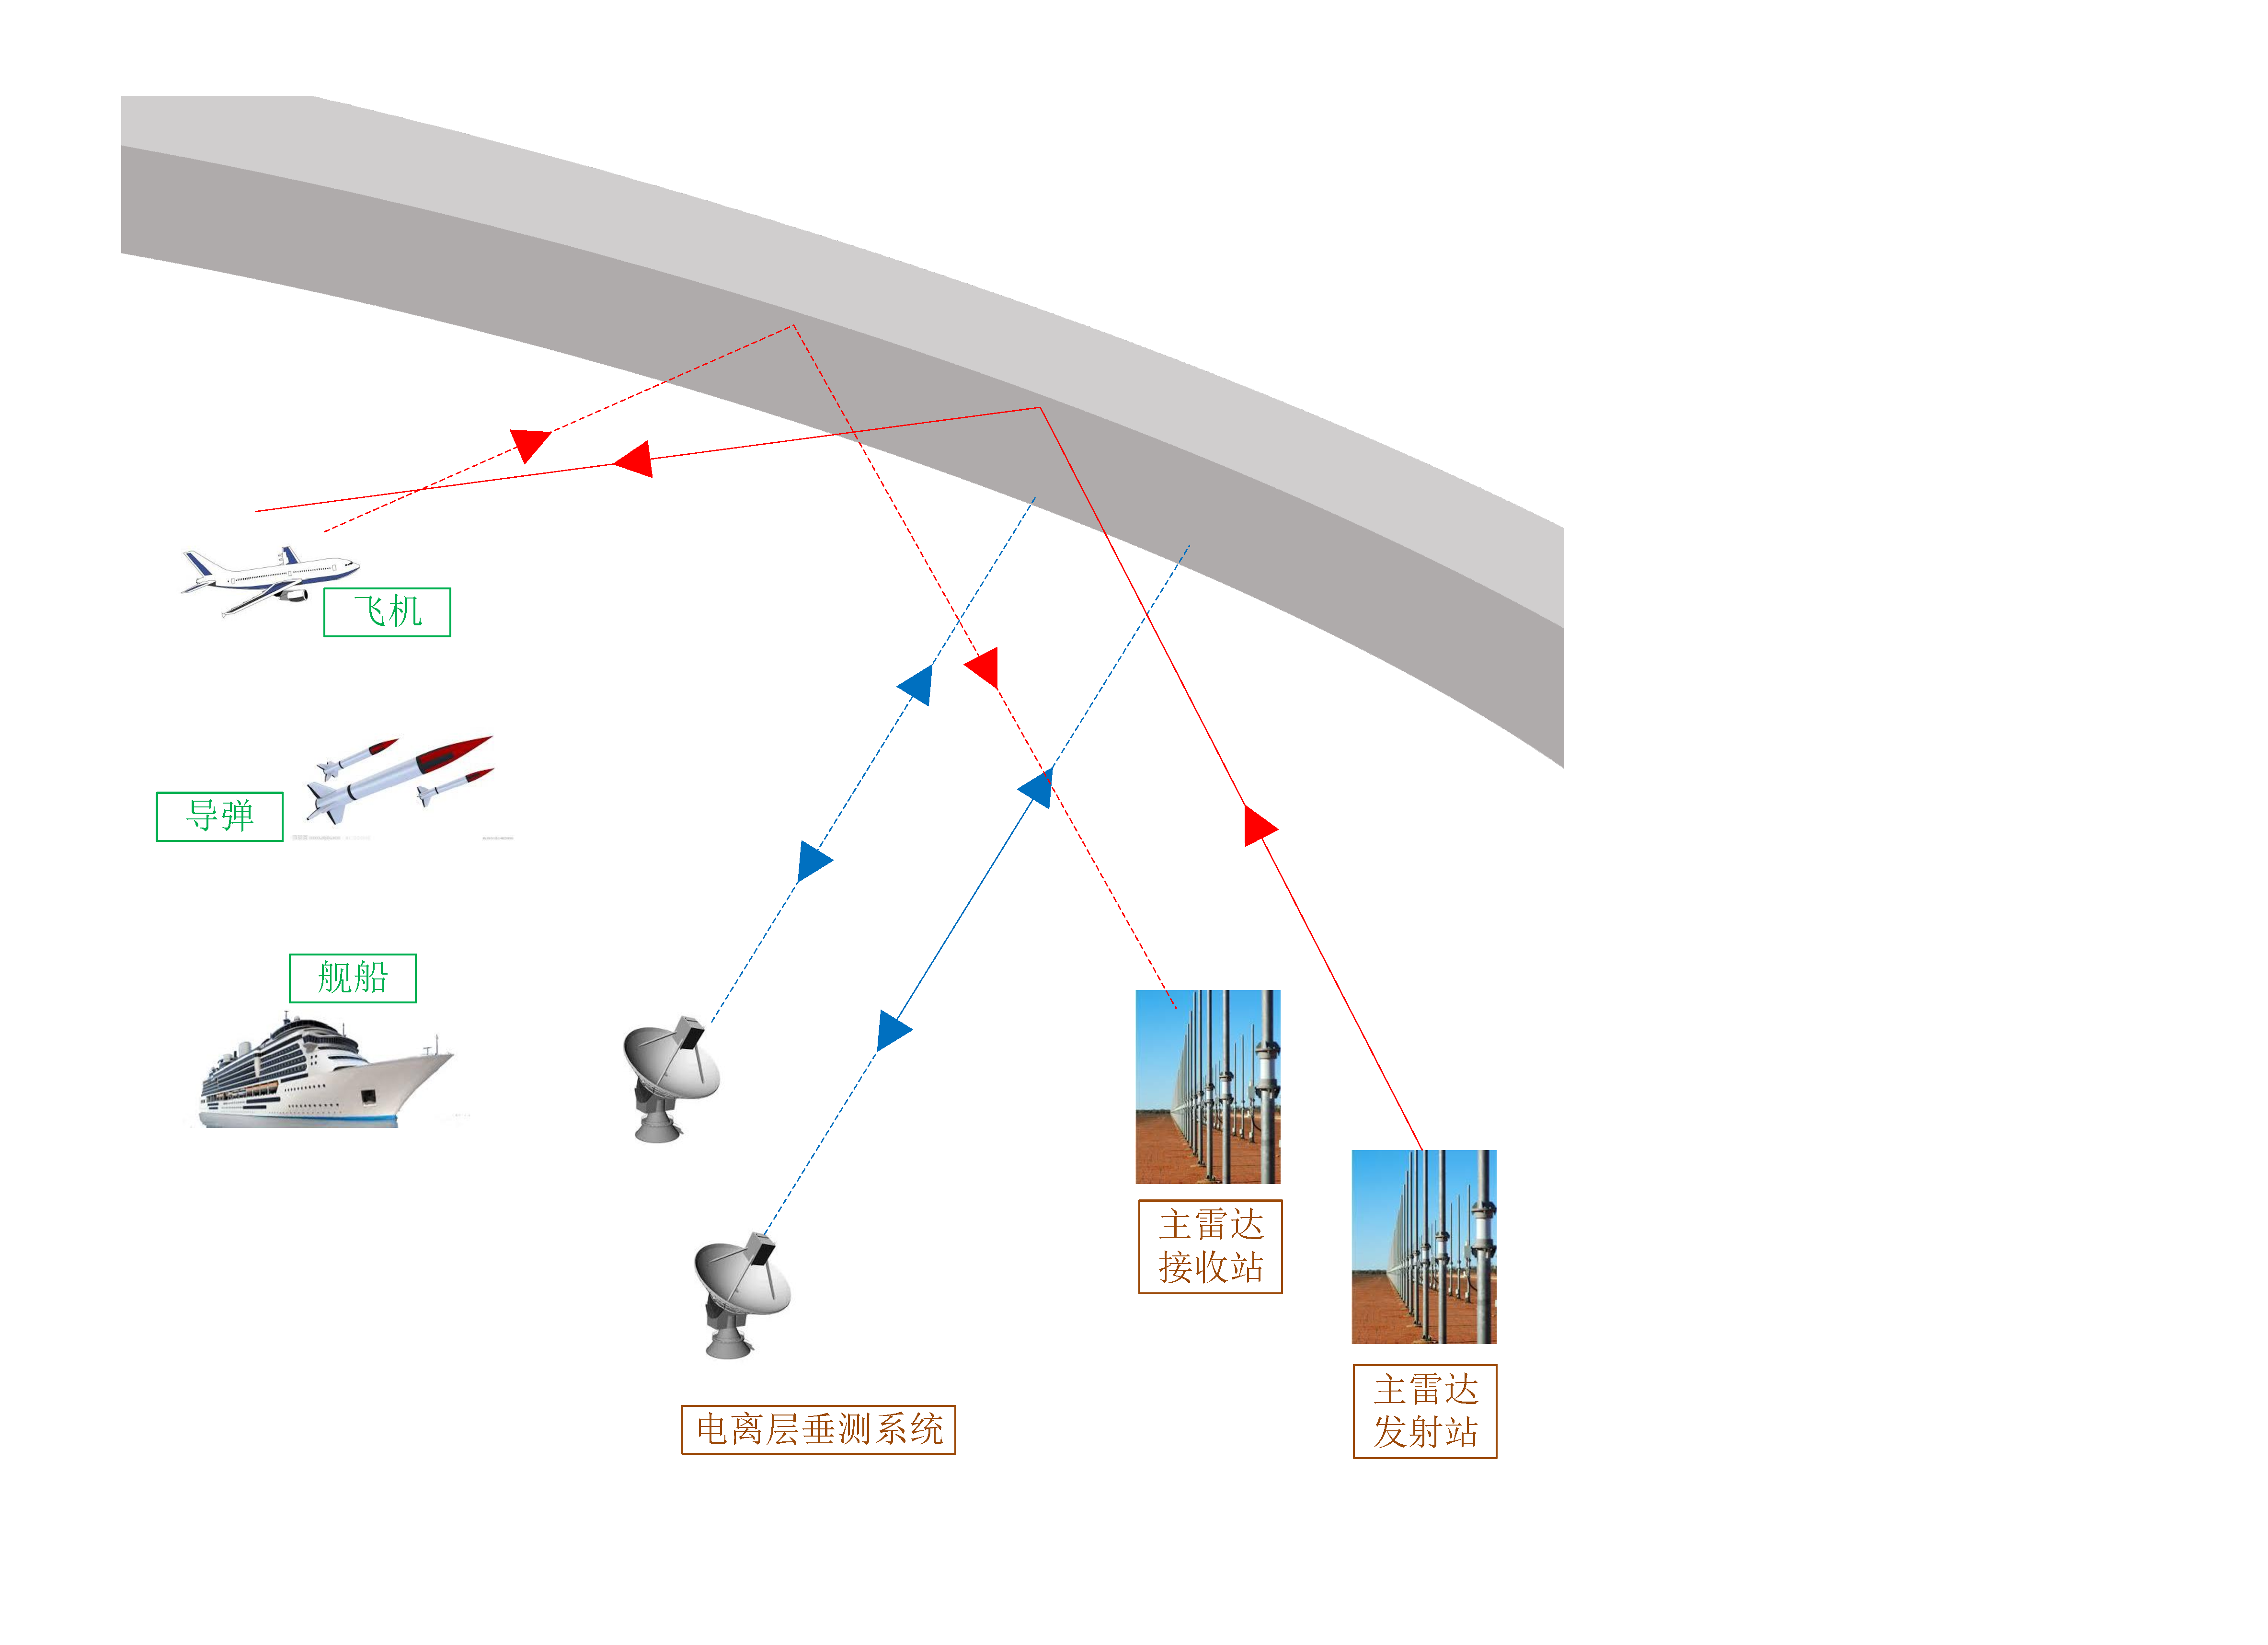
\includegraphics[width=9cm]{figures/introduction/othr_work_new}
	\caption{天波雷达工作原理示意图}
	\label{fig:othr_how}
\end{figure}

天波雷达由于受雷达工作机制及其电波环境的影响,特别是受电离层多模多路径影响,
目标回波-传播模式正确配对很困难,这导致其目标检测和定位精度较低。
如图\ref{fig:pdproblem}所示,天波雷达系统主要由主雷达和电离层探测子系统组成,其中后者为前者提供电离层传播条件评估及坐标配准参数等,如可能的电离层传播模式、每个模式对应的参数或者电离层的每层高度\ucite{wheadon1994ionospheric}。
然而,利用该方法有两个因素会影响目标定位的性能:
第一是探测子系统的部署区域有限,例如该系统无法部署于远海或者敌对区域。对这些不可探测区域的电离层参数通常是建立基于先验信息的电离层统计模型,然后基于统计模型利用已探测区域的参数进行插值求得。但电离层的建模十分复杂且不同区域可能存在较大的变化,这种方式会造成用于坐标配准的电离层参数误差较大,进而影响坐标配准和目标跟踪定位的准确性。
第二是电离层探测子系统独立于主雷达工作导致其提供的坐标配准参数与主雷达不一致,例如电离层探测系统识别的传播模式可能不同于主雷达所接收的量测的传播模式。因此,为了提高电离层传播模式的识别正确率和电离层参数的准确度,进而提高坐标配准的准确性,我们急需研究其它方法。

\begin{figure}[hbt]
\centering
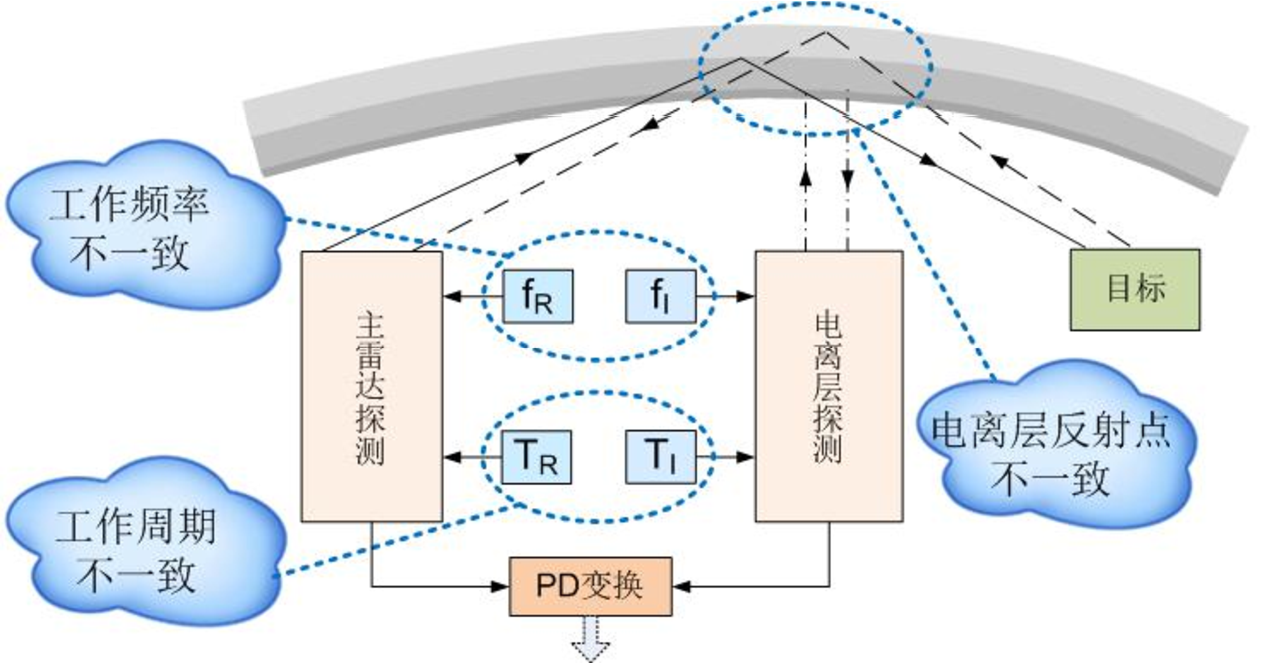
\includegraphics[width=13.5cm]{figures/introduction/pdproblem}
\caption{环境参数(电离层探测系统)与目标参数(主雷达)不一致}
\label{fig:pdproblem}
\end{figure}

针对该问题,传统的解决方法是通过一些辅助检测设备收集信息。
Weijers\ucite{weijers1995oth}提出了一种利用信标来改善坐标配准的方法。
天波雷达接收信标发送的信号,并在雷达坐标系中输出其位置上的量测值。通过将信标的量测与GPS提供的大地坐标系中的位置进行比较,可以实时地进行坐标的校正。然而,这种方法中信标部署区域有限且需要对信标进行维护。

事实上,可以利用远海区域的岛屿作为无源信标来求取电离层的相关参数。如果可以准确的辨识出信号来自陆地还是海洋,可以利用相同的思路进行坐标配准。这种方法的主要思路是,首先通过对频谱数据的分析识别出每个距离方位分辨单元上的地海情况。然后将识别结果中的地海轮廓与先验的地图轮廓信息进行匹配,匹配过程中的偏差可以作为坐标配准的参数。这种方法最重要的一点就是识别出杂波类型,也就是识别出雷达的每一个分辨单元是陆地还是海洋。
这种方法主要有两个优点:一方面是我们可以使用获得的杂波地形图来匹配实际地图,然后根据匹配结果计算偏移量,从而提高目标跟踪的准确性,另一方面,我们可以通过使用由识别结果获得的频谱上的偏移来校正频谱本身,以提高目标检测的概率和准确度。

使用海岸线的坐标配准的想法首先出现在文献\cite{wheadon1994ionospheric}中,然而该文献并没有给出具体的方法以及实际数据的验证。Barnum等人\ucite{barnum1998over}提出了一种基于地海杂波识别的坐标配准方法,主要通过构造杂波模型进行杂波识别。但由于电离层状况的复杂性,地海杂波的特征不稳定(例如海杂波的主要特征布拉格峰可能会偏移甚至失去一个峰值)。

Cuccoli\ucite{cuccoli2009over,cuccoli2009over2,cuccoli2010sea,cuccoli2011coordinate}研究了利用天波雷达监测区域地貌结构来进行坐标配准的方法。
对地理信息中的陆地和海洋用二进制矩阵表示,然后通过等效的电离层反射高度转换为参考信号。通过最大化接收到的雷达回波与地标特征之间的相关性来确定等效的电离层反射高度。然而,他们假设天波雷达传输单脉冲信号且仅提供了数值模拟结果。

Cacciamano等人\ucite{cacciamano2012coordinate}提出了利用3D射线跟踪算法进行坐标配准误差评估的方法。主要思想是通过计算地海分界处的相对群延时与先验已知的实际群延时之间的差异进行坐标配准,其中实际的群延时是通过3D射线跟踪算法得到。Holdsworth\ucite{holdsworth2017skywave} 提出了一种利用地表回波的反向散射强度提高目标定位精度的坐标配准方法。

Fabrizio等人\ucite{fabrizio2016using} 提出了一种使用非合作辐射源在已知参考点产生的雷达回波来提高天波雷达坐标配准精度的方法并使用澳大利亚Jindalee雷达的实验数据对该算法进行了验证。

虽然文献\cite{barnum1998over, weijers1995oth, fabrizio2016using, wheadon1994ionospheric, cuccoli2009over, cuccoli2009over2, cuccoli2010sea, cuccoli2011coordinate, cacciamano2012coordinate}的工作均利用了地理信息进行坐标配准系数的提取,但这些文献的研究重点主要是如何通过地理坐标的匹配来进行坐标配准,而在地海杂波识别方面的研究却并不多。
如图\ref{fig:clutterproblem}所示,天波雷达地海杂波识别面临很多特殊的挑战。首先是杂波模型的复杂度,由于杂波模型随着时间、地点等的变化会发生较大的变化,故杂波建模十分复杂。传统的统计方法中,用于描述雷达杂波的分布有很多种,如瑞利分布(Rayleigh distribution),威布尔分布(Weibull distribution),K分布(K distribution)等,但这些分布均只适用于某些特定情况,而不能在所有情况下均保持良好的效果。
其次,地海杂波的特征无法很好的进行形式化描述。有经验的研究人员可能很容易地根据杂波图区分出某些单元是地还是海,但是用数学方法准确地描述这些特征却非常困难。
\begin{figure}[hbt]
\centering
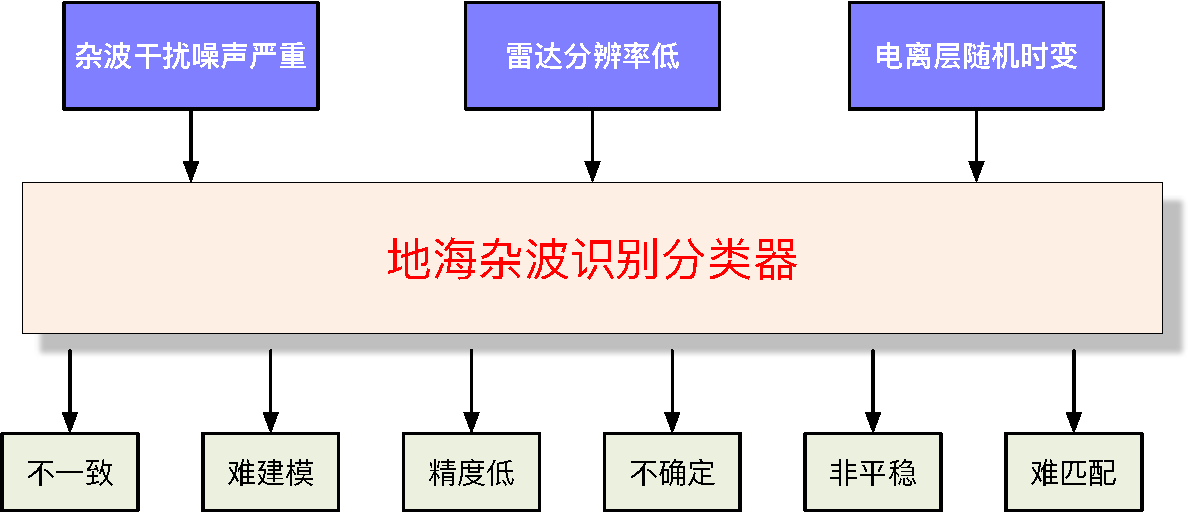
\includegraphics[width=9cm]{figures/introduction/othr_classification.pdf}
\caption{地海杂波识别分类器的背景}
\label{fig:clutterproblem}
\end{figure}

据我们所知,只有Turley\ucite{turley2013high} 和 Jin\ucite{jin2012svm}的工作对地海杂波的识别进行了研究。
文献\cite{turley2013high}定义Bragg Ratio为能量峰值处的多普勒频谱和次高峰处的多普勒频率之比。
利用该统计量在相邻距离方位角单元的基础上构建图边方程(graph edge equations),采用加权最小均方算法(weighted least-mean-square)求解该方程组。
Jin等人\ucite{jin2012svm} 提出了一种基于支持向量机(Support Vector Machine, SVM)的地海杂波识别算法,通过使用三种地海杂波频谱特征来训练SVM,并用仿真数据进行验证,取得了比较好的分类精度。然而,在实际情况下,地海杂波的特征取决于当时的电离层环境等,具有十分强的不确定性,当建模所需的参数变化时,算法的准确性将急剧下降。
如图\ref{fig:othr_tradition}所示,上述两种常规的地海杂波识别算法采用电离层建模、特征提取、分类的方法,但该方法存在电离层建模复杂和信息利用不充分的问题。
\begin{figure}[hbt]
\centering
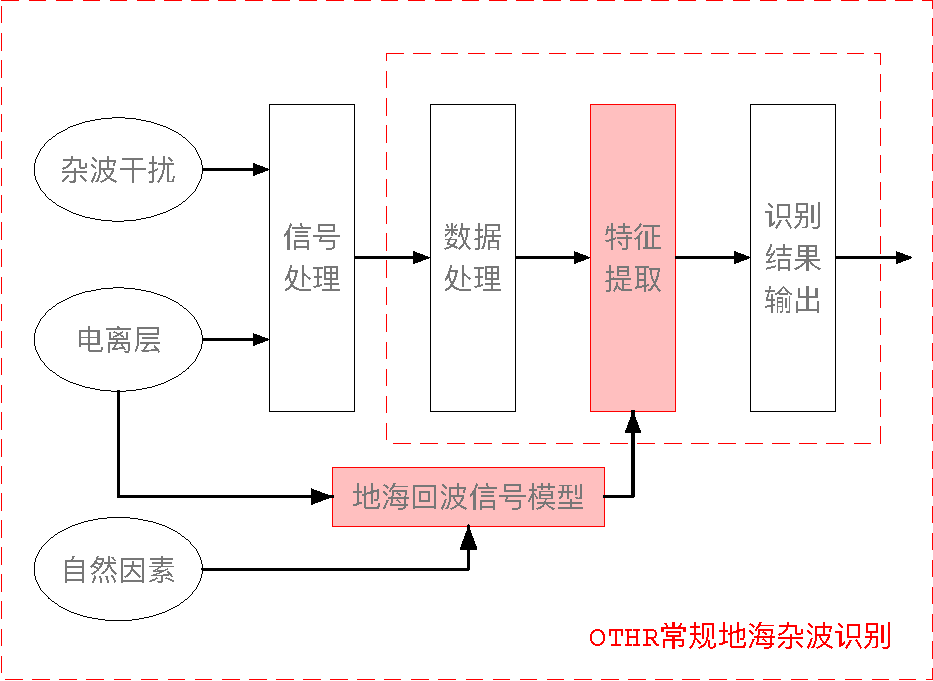
\includegraphics[width=9cm]{figures/introduction/othr_tradition}
\caption{常规地海杂波识别}
\label{fig:othr_tradition}
\end{figure}

\subsection{辐射源个体识别研究现状}
辐射源个体识别(Specific emitter identification, SEI)是一种只依靠接受到的无线信号来辨识出同一型号的辐射源的技术\ucite{Talbot2003Specific}。文献\cite{danev2012physical}阐述了由于射频(radio frequency,RF)电路硬件在生产制造过程中存在公差并且使用过程中使用时间以及工作方式的不同,辐射源个体识别是可以实现的。

随着近几年认知雷达\ucite{kim2008specific}和自组织网络\ucite{zhang2013self}等新技术的出现,
辐射源的快速、准确和鲁棒的自动目标识别在现代军事尤其是军事通讯中的作用日益重要。我国在跟踪发达国家研究进展的基础上也开始加紧研发可装备于军方的SEI系统,以逐步缩小与发达国家在技术实力方面的差距。但总体来说,我国在该方面的研究除了缺乏深层次且系统化的理论分析研究外,更缺乏成熟的工程化系统实践和实际装备,因而迫切需要加快在该领域的理论研究和应用步伐。

辐射源识别是通过将接收信号携带的特征与分类特征组进行比较并选择与这些特征最匹配的类别来区分单个辐射源的过程。
因此,辐射源识别中使用的一种典型方法是维护一个唯一标识各种辐射源信号的特征集,并将辐射源的输入信号与特征集进行比较,并将与输入信号最匹配的特征集的标识符(或标签)分配给它\ucite{Talbot2003Specific,Zanetti2012Exploring}。
这种方法的隐含要求是特征集合,这意味着来自某辐射源个体产生的所有信号的特征值是相似和可重复的,而与由不同辐射源产生的特征值明显不同\ucite{Talbot2003Specific}。
上述分析表明辐射源个体识别的关键技术主要是两部分,一部分是雷达辐射源信号的特征挖掘与提取,另一部分是利用提取的特征进行分类识别。

自上世纪70年代开始,国外很多学者就针对雷达辐射源信号特征挖掘与提取开展了大量研究工作\ucite{therrien1974application},国内的研究始于上世纪80年代初,虽然起步较晚,但受到了军方的高度重视,因此发展迅速。该部分研究主要可以分为两个阶段:

第一阶段为辐射源基本参数特征研究。对原始信号特征直接求取其载波频率、脉冲宽度、脉冲幅度、到达角度和到达时间等信息\ucite{xuxin2001leidajiehuoxitongshishixinhaofenxuanchulijishuyanjiu},选取其中一个或多个作为特征向量。
这种情况主要是应用于电磁环境相对单一、辐射源类别较少、信号形式单一、雷达参数固定的早期。

第二阶段为雷达辐射源信号的脉内特征挖掘。当只利用雷达辐射源的参数无法进行准确的辨识时,
国内外学者开始研究雷达辐射信号的脉内特征,相继提出了多种分析雷达信号脉内特征的方法。
根据辐射源的操作模式,信号可以分为瞬态信号和稳态信号。
瞬态信号,通常被称为开启信号,提供了独特和可区分的特征,适合特征提取和辐射源识别\ucite{choe1995novel,ureten2005bayesian}。测量瞬态特征的主要方法是通过检测噪声的起始点和终点来从噪声中提取瞬态信号\ucite{huang2000bayesian}。一般情况下,辐射源的瞬态特征是特定且一致的,这对识别是十分有帮助的。然而,由于瞬态信号的持续时间非常短,它们很难被捕获。此外,瞬态特征很容易受到非理想和复杂信道条件的阻碍,这可能对识别结果产生负面影响\ucite{xu2007identification}。

稳态信号由在稳定条件下工作的辐射源传输。尽管稳态特征容易被传输的信息破坏而导致提取困难,但由于其很容易被检测和捕获,故稳态信号的识别具有相当大的实际意义。在这种情况下,国内外学者提出了许多特征提取方案,
最先被提出的是对时域信号进行分析处理的方法,如Roe提出的时域波形分析法\ucite{roe1994real};继而学者利用频域信号进行挖掘,如谱相关法\ucite{jouny1995radar,zhang2001new}、脉内瞬时频率特征\ucite{kawalec2004radar,bidaping2005jiyushunshipinlvdemaineidiaozhishibiejishu}与累积法\ucite{aubry2011cumulants}及普运伟提出的瞬时频率派生特征\ucite{puyunwei2009leidafusheyuanxinhaoshunshipinlvpaishengtezhengfenleifangfa},随后学者综合时域信息与频域信息提出了时频综合法\ucite{chen1999joint,li2011quadratic,moraitakis2000feature},时频表示将信号映射到二维时间和频率平面上,同时提供时间和频谱信息。文献\cite{lopez2005digital}基于短时傅立叶变换(short-time Fourier transform, STFT)提出了一个信号检测和识别系统。然而,STFT不能用于分析非线性信号的线性变换。
小波分析因其多分辨率分析的特点也被广泛应用于该领域,Cohen\ucite{cohen2002importance}首次将小波变换引入到信号的分析处理,余志斌在此基础上提出了基于局域波分解\ucite{yuzhibin2008jiyujuyubofenjiedeleidafusheyuanxinhaoshipinfenxi}、小波脊频级联特征\ucite{yuzhibin2010yizhongxinde,yuzhibin2010jiyuxiaobojipinjiliantezhengdeleidafusheyuanxinhaoshibie}的脉内特征挖掘方法和小波包特征\ucite{zhanggexiang2006jiyuxiaobobaobianhuanhetezhengxuanzedeleidafusheyuanxinhaoshibie}等;
越来越多其余学科的知识也被应用于该领域,如信息理论准则与聚类技术综合法\ucite{zhou1999combining}、信号的分形特征\ucite{dudczyk2013identification,zhang2003fractal,dudczyk2013fractal}、基于Chirplet原子的特征\ucite{zhuming2009yizhongjiyu}、熵特征\ucite{zhanggexiang2005jiyushangtezhengdeleidafusheyuanxinhaoshibie}、粗集理论\ucite{zhanggexiang2005jiyucujililundeleidafusheyuanxinhaoshibie}、信息维数\ucite{zhanggexiang2005leidafusheyuanxinhaozhinengshibiefangfayanjiu}和分形盒维数\ucite{zhanggexiang2003leidafusheyuanxinhaofenxingtezhengyanjiu,zhanggexiang2004leidafusheyuanxinhaomaineitezhengfenxi} 等来量化评估信号的不确定性和复杂性。

另一方面,雷达辐射源识别是一个典型的分类问题,其主要思路为在得到辐射源信号的特征表示之后,借助有效的分类算法来实现特征空间到决策空间的转换,从而确定信号的所属类别。
总体上有三种分类方法被应用于雷达辐射源识别中:一种是决策树分类算法,通过人类专家的先验知识进行分类,如ID3\ucite{lyden1999id1}、C4.5算法\ucite{quinlan1996bagging}和模板匹配\ucite{dudczyk2015fast,dudczyk2004applying}等;
另一种为生成模型分类器,其主要是基于先验概率和类别条件概率密度进行估计,如K最近邻算法\ucite{cover1967nearest}。
第三种是判别型分类器,其需要在学习过程中最优化某种目标函数,如线性判别分类器\ucite{mika1999fisher}、神经网络\ucite{jouny1993classification,petrov2013identification,shieh2002vector,willson1990radar}、支持向量机\ucite{ren2008radar}等方法。

从目前的研究现状来看,大多数研究方法存在三个主要缺陷:
\begin{itemize}
\item 特征提取过程计算量大,需要大量的存储空间。
\item 特征选择困难,不同的特征在分类识别能力上存在较大差异。
\item 目前的分类识别局限于已知类别的识别,当有新的来自未知类别的辐射源出现时,无法准确迅速的发现。
\end{itemize}

\subsection{深度学习研究现状}
由于深度学习算法可以有效的学习高维数据的稀疏特征表示,它已经被广泛应用于人脸识别、目标检测、手写字体识别以及场景分类等领域。
1982年,Kunihiko等人\ucite{fukushima1982neocognitron}首次将卷积神经网络(Convolutional Neural Networks, CNN)模型的概念引入神经网络。后来许多学者在实践中对CNN的发展和理论分析作出了重大贡献。1989年,LeCun等人将基于梯度的学习方法\ucite{lecun1998gradient}和BP算法\ucite{lecun1989backpropagation}引入到卷积神经网络。2003年,Behnke写了一本总结卷积神经网络\ucite{behnke2003hierarchical}的书。同年,Simard等人\ucite{simard2003best}对卷积神经网络进行了简化。2011年,Ciren等\ucite{ciresan2011flexible}进一步改进卷积神经网络并实现了GPU版本,使得卷积神经网络的训练识别速度有了巨大的提升,并使用卷积神经网络框架对多个图像数据库进行实验,并取得了最佳成果。

深度学习在无监督分类领域的研究也十分广泛,Hinton和PDP小组\ucite{rumelhart1985learning}于20世纪80年代首次提出自编码器这种对输入数据进行重构的神经网络结构,用输入数据作为标签来解决无监督反向传播的问题。
自编码器与Hebbian学习规则\ucite{hebb2005organization}共同为无监督学习提供了一个基本的范例,后来被推广到各种问题的全局学习方面。
自编码器在深度架构方法中占据着比较重要的位置,特别是形式上类似受限玻尔兹曼机的自编码器,堆栈自编码器。堆栈自编码器通过首先利用无监督的方式自下而上地进行训练,随后是以有监督学习的方式训练顶层并微调整个架构,在一些具有挑战性的分类或回归问题上得到了最好的结果\ucite{hinton2006reducing,hinton2006fast,bengio2007scaling,erhan2010does}。

由于深度学习算法在图像、语音等领域的卓越表现,一部分学者也开始将其应用于雷达领域。在研究初期,大部分应用均集中于合成孔径雷达(Synthetic aperture radar, SAR)图像识别,主要用于遥感中的地物分类领域。
Chen\ucite{chen2014sar}提出了一种利用单层卷积神经网络从SAR图像自动学习特征进行分类的方法,并利用MSTAR公开数据集进行验证得到了较高的分类准确率。
Lv\ucite{lv2014classification}提出了一种基于深度置信网络的城市测绘方法,在复杂的城市环境中仍可以保持很高的精度,优于自适应支持向量机等方法。
Xie\ucite{xie2014multilayer}提出了一种自动学习极化合成孔径雷达(PolSAR)中多层特征的方法,首先利用堆栈稀疏自编码器进行特征提取,然后使用少量标签微调方法中的参数,显著提升了分类精度。

而随着深度学习技术的发展,一部分学者逐渐把深度学习引入新的领域。恒虚警(Constant False Alarm Rate, CFAR)检测是雷达系统常用的目标检测算法,Rohman\ucite{rohman2017classification}提出了一种隐含神经元数变化的集成神经网络分类器,对雷达环境进行分类的自适应CFAR检测方法。在多目标和杂波边界环境下,该方法仍然能够表现出最好的性能。Kim\ucite{kim2016human}提出了一种基于多普勒雷达的深度卷积神经网络(DCNNs)用于人体检测和活动分类的方法。 他们主要针对传统解决方案中依赖手工特征设计的问题,提出了将DCNN直接应用于人体检测和活动分类问题的原始多普勒频谱图。DCNN可以使用量测数据共同学习必要的特征和分类边界,而不需要在多普勒信号上使用任何明确的特征,并且取得了很高的精度。
Zhang\ucite{zhang2017novel}针对不同运动形式和复杂杂波背景下的多目标跟踪问题,通过将传统的MN逻辑航迹起始算法与深度学习进行结合实现了在复杂杂波环境下的多目标航迹起始算法。仿真实验表明,其方法比传统的用于航迹起始的改进Hough变换要好得多,特别是在目标机动的情况下,同时该方法具有很强的鲁棒性和适应性,能够对来自不同雷达的数据进行起始。
% 虽然深度学习算法在雷达信号分类识别中的应用场景逐渐增大,但是大部分的实施步骤仍然是利用二维的卷积神经网络对图像进行分类识别。


\section{论文研究内容及结构}

本文基于深度学习方法,研究其在复杂环境下的天波雷达地海杂波识别和含有未知分类的辐射源分类中的应用。本文各章安排如下:

第\ref{sec:intro}章为绪论,主要介绍了天波雷达地海杂波识别的意义与发展,辐射源类别识别以及深度学习方法在雷达信号分类领域的国内外研究现状。

第\ref{sec:network}章为深度卷积神经网络。该章详细介绍深度学习理论。

第\ref{sec:othr}章为基于深度学习的地海杂波识别。该章根据天波雷达的频谱信息,构建了一个深度卷积神经网络分类器,
作为分类器区分出获取的杂波类型。验证结果表明,即使是在电离层环境很差的情形下,该算法仍然具有很高的精确度。
并且将识别结果与实际的地图轮廓进行了匹配,仍然具有很高的匹配率。

第\ref{sec:decc}章基于深度嵌入卷积聚类方法的地海杂波无监督分类。结合卷积神经网络与自编码器提出了一种无监督分类算法,深度嵌入卷积聚类方法。利用卷积自编码器进行特征提取,并在损失函数中将KL散度与重构损失两部分结合,并利用天波雷达地海杂波数据进行了测试,结果验证了深度嵌入卷积聚类算法的有效性。

第\ref{sec:sei}章为基于深度学习的辐射源未知分类识别。针对复杂电磁环境下辐射源识别困难的问题,设计了一个深度卷积神经网络,利用模糊函数作为特征实现了对已知类别的辐射源的识别。同时设计了一个Meta-Recognization,对识别结果做进一步处理,实现了未知分类的辨别。利用来自多架飞机气象雷达的实际数据进行了测试,实验结果验证了本文提出的算法具有很高的识别准确率和未知分类分辨正确率。

第\ref{sec:paper_summary}章对全文进行总结,并对后续的研究方向进行了讨论。
